\documentclass[a4paper,11pt,twoside]{article}
%\documentclass[a4paper,11pt,twoside,se]{article}

\usepackage{UmUStudentReport}
\usepackage{verbatim}   % Multi-line comments using \begin{comment}
\usepackage{courier}    % Nicer fonts are used. (not necessary)
\usepackage{pslatex}    % Also nicer fonts. (not necessary)
\usepackage[pdftex]{graphicx}   % allows including pdf figures
\usepackage{listings}
\usepackage{pgf-umlcd}
%\usepackage{lmodern}   % Optional fonts. (not necessary)
%\usepackage{tabularx}
%\usepackage{microtype} % Provides some typographic improvements over default settings
%\usepackage{placeins}  % For aligning images with \FloatBarrier
%\usepackage{booktabs}  % For nice-looking tables
%\usepackage{titlesec}  % More granular control of sections.

% DOCUMENT INFO
% =============
\department{Department of Computing Science}
\coursename{Object-Oriented Programming Methodology 7.5 p}
\coursecode{5DV133}
\title{OU4 Sensor Network}
\author{Johan Eklund ({\tt{kv03jed@cs.umu.se}}) \\ 
Tommie Lindberg ({\tt{c15tlg@cs.umu.se}}) \\
Jakob Lundin ({\tt{c14jln@cs.umu.se}}) \\
Lorenz Gerber ({\tt{dv15lgr@cs.umu.se}}, {\tt{lozger03@student.umu.se}})
}
\date{2016-05-23}
%\revisiondate{2016-01-18}
\instructor{Anders Broberg \\ Niklas Fries \\ Adam Dahlgren \\
  Jonathan Westin \\ Erik Moström \\ Alexander Sutherland}


% DOCUMENT SETTINGS
% =================
\bibliographystyle{plain}
%\bibliographystyle{ieee}
\pagestyle{fancy}
\raggedbottom
\setcounter{secnumdepth}{2}
\setcounter{tocdepth}{2}
%\graphicspath{{images/}}   %Path for images

\usepackage{float}
\floatstyle{ruled}
\newfloat{listing}{thp}{lop}
\floatname{listing}{Listing}



% DEFINES
% =======
%\newcommand{\mycommand}{<latex code>}

% DOCUMENT
% ========
\begin{document}
\lstset{language=C}
\maketitle
\thispagestyle{empty}
\newpage
\tableofcontents
\thispagestyle{empty}
\newpage

\clearpage
\pagenumbering{arabic}

\section{Introduction} 
The assignment was described on the course homepage
\cite{sensornetwork}. The main aim idea was to develop software that
allows to perform experiments on sensor networks as described in
Braginsky and Estrin \cite{braginsky2002}. The main topic of
\cite{braginsky2002} is the use of \textit{rumour routing} as an
energy saving message transportation algorithm that for example
be used in environment surveillance networks.

In object oriented software design, it is common to build 
a model representation of the real world system \cite{roleplay} by
defining classes the correspond to the real world systems' entities.  
Here the real world system is a sensor network as described in
Braginsky and Estrin \cite{braginsky2002}. The realworld entities
modelled in this assignment can be classified in two main groups: Physical
components such as the sensor nodes and non-physical ones, information packages
travelling the network, such as the queries and agents. Further, a third type, 
the environment entity simulates the real surrounding.

\textit{Unified Modelling Language} (\textit{UML}) diagrams were
composed according to Börstler \cite{roleplay}. The theory of rumour
routing is described by Braginsky \cite{braginsky2002}. Horstman was
used as Java language reference \cite{horstman2014} for chosing datatypes.

\section{Compiling and Running of the Program}

\subsection{Javadoc}


\section{Description of Program Structure}
\subsection{Specific Design Decisions}
Figure \ref{fig:uml} shows the UML diagram of the chosen design. 
\begin{figure}
\centering
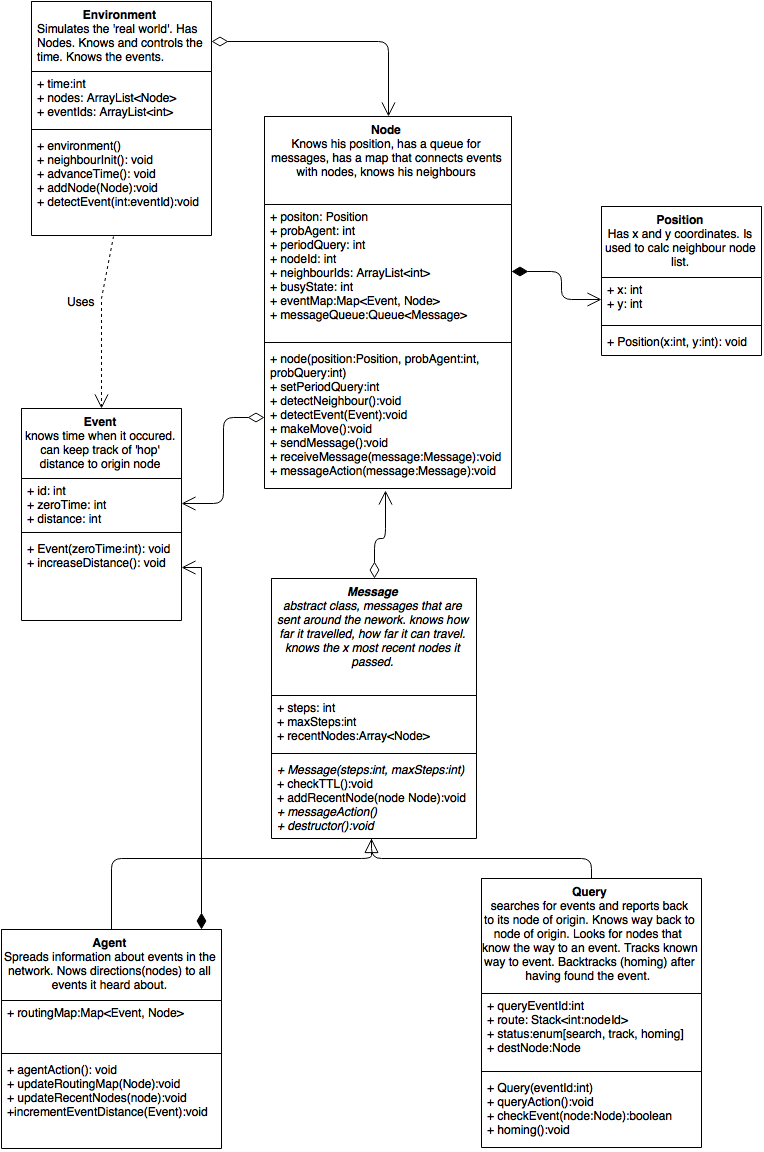
\includegraphics[width=\textwidth]{uml.png}
\caption{\textit{UML diagram for implementing a sensory network application
  that allows testing of the rumour routing algoritm.}}
\label{fig:uml}
\end{figure}

\subsection{Initialization and State Stepping}
We define our variables to fit the specifications, then constructs an
environment class. The program then iterates through every node,
giving them each a position, such that they align as a grid. Four
random nodes are given a value for periodQuery, making them the query
origin nodes. To create a neighbour list, we iterate through every
node, checking distance to each node and storing the nodes in
reachable distance in the Node.neighbors list. 
After this, the network is initialised and we loop the
myEnv.advanceTime() function to run the program.

\subsection{Environment Class}
The Environment class stores information in the network, stores nodes,
keeps track of events, and controls time. It is the simulation
environment, which simulates the ‘real world’. The advanceTimer() lets
each node make a “move”, sending a message if there is a message in
its queue.

\subsection{Node Class}
The Node class stores information about specific nodes, such as
position, neighbouring nodes, and paths to events. The nodes also send
and receive messages. Each time the makeMove() method is called, the
detectEvent() method “rolls a die” to see if an event will be created
on the node. If there is an event, there is a chance of an agent being
created, according to the specified probability. If it is one of the
query origin nodes, it checks the queryPeriod. If 0, it creates a new
query and puts it on queue. If its BusyState is false, it will send a
message from its queue. When a message is sent, the method checks to
see what type of message it’s trying to send. If the message is a
query, it then checks the query state to see where it should be
sent. It then checks if the intended receiver is free, if not, the
message is sent. The method recieveMessage adds the incoming message
to its queue called messageQueue. It will then set the node in
busyState so that the node can’t receive any more messages this
timestep. If the message is received from an agent it will increment
the events distance with one.


\subsection{Classes Message, Query and Agent}
The Message class is an abstract class and will use the abstract
method messageAction. This will be used so that the node don’t need to
determine if the message is an agent or query.

The Query class extends message and will call to the public method
queryAction. The queryAction will first check which mode is
initialised for the query. The query has three different mode setups,
the search, track and homing mode. When the query is in search mode it
will step through the nodes in the routingMap and all the steps is
inserted in a stack called route. It will look in each nodes eventMap
until it finds the unique eventId it is set to find. If the eventId is
found the query switches to track mode.
Track mode is used to find the unique events origin. It will track
through the neighbours to the node where the event first was found
until it finds where the event distance is zero. When the origin of
the event is found it will store the node in destNode and it switches
mode to homing.
Homing mode is used to track back the same way it went to the start
node. The query will use the stack route to find the exact way it
stepped until the stack is empty.
It will then exclaim the events position, the time the event happened
and which node caught the event.

The Agent class extends message and will call to the public method
agentAction. The queryAction will compare it’s eventMap with the nodes
eventMap. If they are not alike the node will add the differences to
it’s own eventMap. The agent will then check it’s time to live. If the
time to live is zero the agent will not step to another node. If it's
not zero it will decrement it’s time to live before it steps to
another node.

\section{Testing Framework}
The program will be tested with both JUnit tests for methods and
smaller programs to test the functionality of the different classes.
During the building of the classes we will use JUnit tests, to make
sure the constructors and methods work properly. We will also use
different exceptions and try and catch methods because that will make
it easier for us to determine and find where something goes wrong in
the code. When the building of a class is completed we are going to
build a small program that we know only will get one result if it
works as we expect. This program will be used on the finished class so
we know that it works and we get the results we want out of the
class. When all the classes are built and tested we will put them
together to a complete program and some easier tests will be made for
the program so we know it’s stable and works as we want.  

\addcontentsline{toc}{section}{\refname}
\bibliography{references}

\end{document}
 
